
\section{Introduction}


\begin{figure}[b]
\begin{center}
\vspace{-0.5cm}
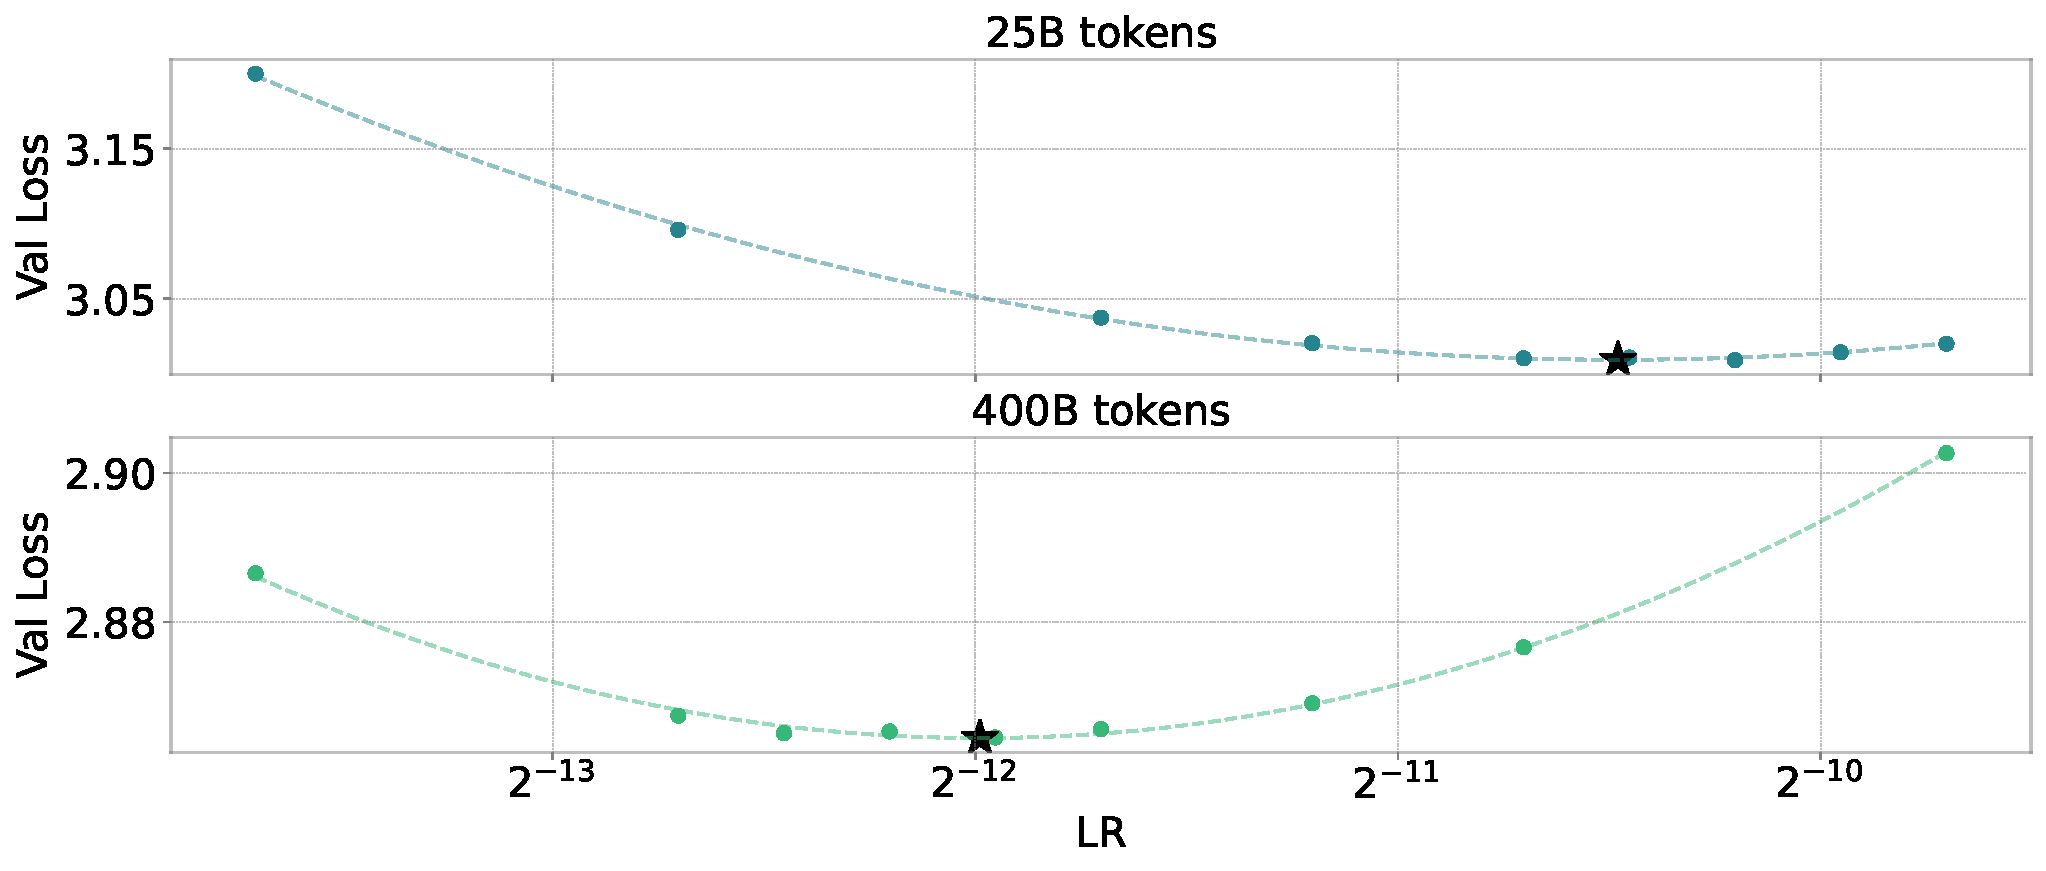
\includegraphics[width=0.85\textwidth]{images/teaser_350m.pdf}
\vspace{-0.3cm}
\caption{Final validation loss of a 350 million parameter LLM for different learning rates (LR) and token horizons. The dashed lines indicate our fitted curve and the stars indicate the estimated optimal LR. The optimal LR decreases as the token horizon increases.}
\label{fig:350m_teaser}
\centering
\end{center}
\end{figure}


State-of-the-art LLMs are scaled in multiple dimensions. The models are becoming increasingly large, e.g. Grok-1.5 has 314 billion (B) parameters \citep{grok1_release}. The clusters used to train them are growing in size, e.g. the recently operational Memphis super-cluster contains over 100,000 H100 GPUs \citep{musk_ai_cluster_2024}. Lastly, the training datasets are growing, e.g. LLama-3 was trained on 15 Trillion (T) tokens \citep{llama3}. At these scales, it is infeasible to extensively tune hyperparameters. Practitioners must instead resort to \textit{hyperparameter transfer}, a process where approximately optimal hyperparameters for large-scale experiments are inferred from experiments at a smaller scale. Perhaps the most famous work on hyperparameter transfer is muP \citep{mup} -- a methodology for transferring optimal hyperparameter from a small model to a large model. While hyperparameter transfer across model size is a well-studied problem, transfer across token horizon remains understudied. This paper aims to remedy this shortcoming in the literature. 

In this paper, we present a large-scale study on hyperparameter transfer across token horizons, we define the latter as the total number of tokens seen during training. We specifically focus on learning rate (LR), an important hyperparameter that influences training stability, generalization, and convergence speed. Our study is essentially a large ablation experiment where we vary LR and token horizon for a few different LLM models. We consider $>$250 training runs in total. To keep the scope and computational requirements manageable we focus on how LR depends on the token horizon, and only present some preliminary results on its interaction on model size. Our experiments are based on standard public resources -- the Megatron codebase \citep{shoeybi2019megatron} and the RefinedWeb dataset \citep{refinedweb}. Our three main contributions are:



\begin{itemize}
    \item We provide a large-scale study demonstrating that the optimal LR depends strongly on the token horizon, with longer horizons necessitating smaller LRs. This fact holds even when muP parametrization is used.
    \item We demonstrate that 1) the optimal LR for any given architecture follows a scaling law and 2) this allows \textit{hyperparameter transfer} where the optimal LR for a long horizon is inferred from a shorter horizon. Furthermore, we provide a rule-of-thumb for transferring LR across token horizons with zero overhead over current practices.
    \item We provide a case study on the optimal LR for the LLama architecture. We provide evidence that LLama-1 used an LR that is too large, highlighting hyperparameter transfer across horizons as an overlooked component of LLM training. 
\end{itemize}


